%%%%%%%%%%%%%%%%%%%%%%%%%%%%%%%%%%%%%%%%%
% Beamer Presentation
% LaTeX Template
% Version 1.0 (10/11/12)
%
% This template has been downloaded from:
% http://www.LaTeXTemplates.com
%
% License:
% CC BY-NC-SA 3.0 (http://creativecommons.org/licenses/by-nc-sa/3.0/)
%
%%%%%%%%%%%%%%%%%%%%%%%%%%%%%%%%%%%%%%%%%

%----------------------------------------------------------------------------------------
%	PACKAGES AND THEMES
%----------------------------------------------------------------------------------------

\documentclass{beamer}

\mode<presentation> {

% The Beamer class comes with a number of default slide themes
% which change the colors and layouts of slides. Below this is a list
% of all the themes, uncomment each in turn to see what they look like.

%\usetheme{default}
%\usetheme{AnnArbor}
%\usetheme{Antibes}
%\usetheme{Bergen}
%\usetheme{Berkeley}
%\usetheme{Berlin}
%\usetheme{Boadilla}
%\usetheme{CambridgeUS}
%\usetheme{Copenhagen}
%\usetheme{Darmstadt}
%\usetheme{Dresden}
%\usetheme{Frankfurt}
%\usetheme{Goettingen}
%\usetheme{Hannover}
%\usetheme{Ilmenau}
%\usetheme{JuanLesPins}
%\usetheme{Luebeck}
%\usetheme{Madrid}
%\usetheme{Malmoe}
%\usetheme{Marburg}
%\usetheme{Montpellier}
%\usetheme{PaloAlto}
%\usetheme{Pittsburgh}
%\usetheme{Rochester}
%\usetheme{Singapore}
%\usetheme{Szeged}
\usetheme{Warsaw}

% As well as themes, the Beamer class has a number of color themes
% for any slide theme. Uncomment each of these in turn to see how it
% changes the colors of your current slide theme.

%\usecolortheme{albatross}
%\usecolortheme{beaver}
%\usecolortheme{beetle}
\usecolortheme{crane}
%\usecolortheme{dolphin}
%\usecolortheme{dove}
%\usecolortheme{fly}
%\usecolortheme{lily}
%\usecolortheme{orchid}
%\usecolortheme{rose}
%\usecolortheme{seagull}
%\usecolortheme{seahorse}
%\usecolortheme{whale}
%\usecolortheme{wolverine}

%\setbeamertemplate{footline} % To remove the footer line in all slides uncomment this line
%\setbeamertemplate{footline}[page number] % To replace the footer line in all slides with a simple slide count uncomment this line

%\setbeamertemplate{navigation symbols}{} % To remove the navigation symbols from the bottom of all slides uncomment this line
}

\usepackage{graphicx} % Allows including images
\usepackage{booktabs} % Allows the use of \toprule, \midrule and \bottomrule in tables

%----------------------------------------------------------------------------------------
%	TITLE PAGE
%----------------------------------------------------------------------------------------
\title[Cache Oriented Obfuscation]{Obfuscating Malware through Cache Memory Architecture Features} % The short title appears at the bottom of every slide, the full title is only on the title page

\author{Caglar Sayin} % Your name
\institute[HIG] % Your institution as it will appear on the bottom of every slide, may be shorthand to save space
{
Gjovik University, Norwegian Information Security Laboratory \\ % Your institution for the title page
\medskip
\textit{me@caglarsay.in} % Your email address
}
\date{Oct 15, 2014} % Date, can be changed to a custom date

%----------------------------------------------------------------------------------------
%	PRESENTATION Begins
%----------------------------------------------------------------------------------------

\begin{document}

\begin{frame}
\titlepage % Print the title page as the first slide
\end{frame}



%----------------------------------------------------------------------------------------
%	PRESENTATION SLIDES
%----------------------------------------------------------------------------------------

\begin{frame}
	\frametitle{What do we propose?}
	\Large
	Highly advanced APT Obfuscation method through cache memory features which can be availably empowered by complexity of concurrency.
\end{frame}


\begin{frame}
	\frametitle{Generalization vs Specification}
	\Large
	More than generalization, based on specification. 
\end{frame}

\begin{frame}
	\frametitle{Generalization vs Specification}
		\begin{figure}
			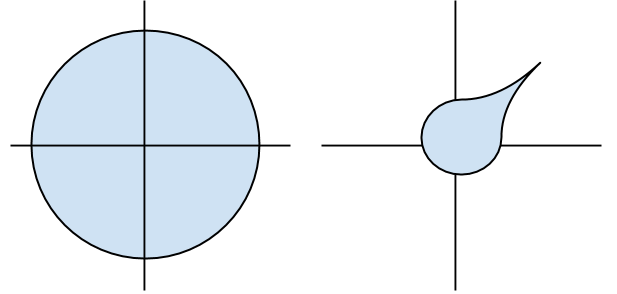
\includegraphics[width=0.8\linewidth]{img/spvsgn.png}
		\end{figure}
\end{frame}


%------------------------------------------------

\begin{frame}
\frametitle{Overview} % Table of contents slide, comment this block out to remove it
\setcounter{tocdepth}{1}

\tableofcontents % Throughout your presentation, if you choose to use \section{} and \subsection{} commands, these will automatically be printed on this slide as an overview of your presentation
\end{frame}

%------------------------------------------------
\section{Background Studies} 
%------------------------------------------------

\begin{frame}
	\frametitle{What are you going to point out, today?}
	\begin{itemize}
		\item Malware Obfuscation
		\item Taxonomy
		\item Promising Issues
		\item Their Countermeasures
		\item Cache and Memory Architecture Features
		\item Our Methods
	\end{itemize}
\end{frame}

%------------------------------------------------
\subsection{Obfuscation mechanisms}
%------------------------------------------------

\begin{frame}
	\frametitle{Code Obfuscation}
	\begin{itemize}
		\LARGE
		\item Stub-Body-Tail Based Obfuscations
		\item Control Flow Obfuscation
	\end{itemize}
\end{frame}

%------------------------------------------------
\begin{frame}[plain]
	\frametitle{Stub-Body-Tail Based Obfuscations - Polymorphism}
	\begin{columns}[c] % The "c" option specifies centered vertical alignment while the "t" option is used for top vertical alignment

\column{.70\textwidth} % Left column and width
\begin{description}
	\small
	\item[Stub] Deobfuscate and obfuscate code. Detectable because of being plain text.
	\item[Body] Payload, and it is obfuscated code.
	\item[Tail] Regeneration stub section for next time.
\end{description}

\column{.5\textwidth} % Right column and width
	\begin{figure}
		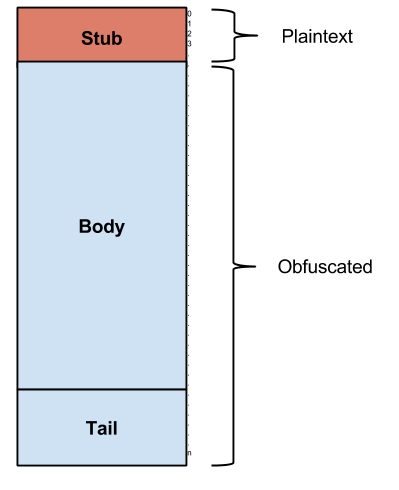
\includegraphics[width=1\linewidth]{img/code_illustration.png}
	\end{figure}
\end{columns}
\end{frame}

%------------------------------------------------

\begin{frame} 
\frametitle{Control Flow Obfuscation - Metamorphism}
\begin{itemize}
\item Register Swaping
\item Register Exchanging
\item Filling NOP instruction randomly
\item Build code semantic with JMP or CALL Instructions
\item Independent Code Order Exchanging 
\item Inserting junk codes and loops
\end{itemize}
\end{frame}

%------------------------------------------------
\begin{frame}[plain, fragile] 
\frametitle{Control Flow Obfuscation - Metamorphism}
Task f(x) = 10 * sin(2 * x)
\begin{example}[Payload Code]
	\begin{verbatim}
		t = x
		t = t * 2
		t = sin(t) 
		t = t * 10\end{verbatim}
	\end{example}
\end{frame}

%------------------------------------------------

\begin{frame}[plain, fragile] 
\frametitle{Control Flow Obfuscation - Metamorphism}
Task f(x) = 10 * sin(2 * x), and lets change a bit order
\begin{example}[Payload Code]
	\begin{verbatim}
		t = 2 * x 
		a = sin(t) 
		t = 10 * a\end{verbatim}
	\end{example}
\end{frame}

%------------------------------------------------

\begin{frame}[plain, fragile] 
\frametitle{Control Flow Obfuscation - Metamorphism}
Task f(x) = 10 * sin(2 * x), but it is semantically equal to f(x) = sin(x)*cos(x)*20, so
\begin{example}[Payload Code]
	\begin{verbatim}
		t = x
		a = sin(t)
		b = cos(t)
		t = a * b
		t = t * 20\end{verbatim}
	\end{example}
\end{frame}

%------------------------------------------------

\begin{frame}[plain, fragile] 
\frametitle{Control Flow Obfuscation - Metamorphism}
Task f(x) = sin(x)*cos(x)*20, and we can change a bit order while preserving semantic
\begin{example}[Payload Code]
	\begin{verbatim}
		b = cos(x)
		t = 20 * b
		a = sin(x)
		t = t * a\end{verbatim}
	\end{example}
\end{frame}

%------------------------------------------------

\begin{frame} % Need to use the fragile option when verbatim is used in the slide
\frametitle{Hybrid Approach}
\begin{itemize}
	\item It is basically Polymorphic Obfuscation.
	\item Stub part is obfuscated with metamorphism by tail section.
	\item It is one of the most common method with APT malware.
	\item They both empower each other's weakness.
\end{itemize}
\end{frame}

\begin{frame} % Need to use the fragile option when verbatim is used in the slide
\frametitle{On the Other Side of the Coin}
\begin{itemize}
	\item Obfuscation function is totally rocket science
	\item Indistinguishability Obfuscator Function Proposed by Garg Et.al.
	\item This function are also implementable for functional encryption.
	\item Homomorphic Functions looks like promising.
	\item Most of the Practical Examples are using XOR :).
\end{itemize}
\end{frame}

%------------------------------------------------
\subsection{In-memory hiding techniques}
%------------------------------------------------

\begin{frame}
	\frametitle{In-memory hiding techniques}
	\begin{block}{TLB Splitting}
		Desynchronizing separated TLBs in the same system(DATA TLB and Instruction TLB). It is really useful for Rootkit to conceal specific region from read operations. 
	\end{block}

	\begin{block}{Architecture and OS Related MMU Evasion Methods}
		\small{Because of the lack of privileged architecture of HW or OS, anybody can access control instructions, also the rootkit which works on kernel mode can access control instructions of MMU. Then, They can create their own NUMA - private memory sections. }
	\end{block}

	\begin{block}{Time of Check, Time of Use attack}
		Driver Jumping Attack is one of the example of this kind.
	\end{block}
\end{frame}

%------------------------------------------------

%------------------------------------------------
\subsection{Multi-Processing Malware Approach}
%------------------------------------------------
\begin{frame}
	\frametitle{Multi-Processing Malware Approach}
	\begin{itemize}
		\item Multi-Processing Malware has extreme detection cost in concurrent architectures
		\item The common aspect is stitching lots of benign code in a semantic order
		\item Concurrent malware processing require concurrent memory observation
		\item Concurrent memory observation cost increases exponentially.
		\item It is pretty hot field for security researchers
	\end{itemize}
\end{frame}

%------------------------------------------------
\subsection{Detection of Obfuscated Malware}
%------------------------------------------------

\begin{frame}
	\frametitle{Detection of Obfuscated Malware}
	\begin{itemize}
		\item Control Flow and Data Flow Graphs
		\item Entropy Analysis
		\item Dynamic Methods Like Emulating, Debugging, Sandboxing
		\item Behavioural Analysis
		\item Memory Inspection
	\end{itemize}
\end{frame}

\begin{frame}
	\frametitle{Memory Inspection}
	\begin{itemize}
		\item Polymorphism is weak against memory inspection because it is disk to memory obfuscation.
		\item Most of the rootkit scanners are based on memory inspection
		\item If you switch off TLB usage during inspection, It can solves TLB splitting
		\item Hardware Based Memory Inspector getting common (e.g CoPilot, GPU based example by C. Tsopokis)
		\item it is still not combined with dynamic approaches or real time approach
	\end{itemize}
\end{frame}

%------------------------------------------------


%------------------------------------------------
\section{Cache Oriented Obfuscation}
%------------------------------------------------
\begin{frame}
	\frametitle{The First Answer}
	\huge{\centerline{Cache Oriented Obfuscation}}
\end{frame}

%------------------------------------------------
\begin{frame}
	\frametitle{Tightly Coupled Memory Systems}
		\begin{figure}
			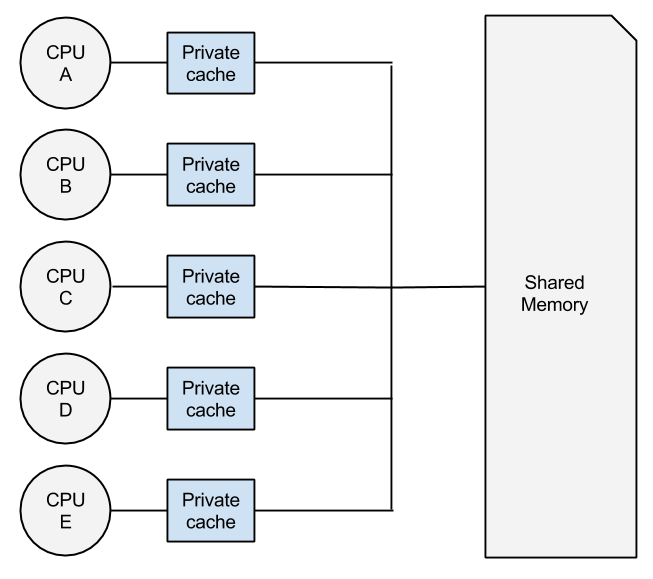
\includegraphics[width=0.6\linewidth]{img/tightly_coupled_memories.png}
		\end{figure}
\end{frame}

%------------------------------------------------

\subsection{Cache Memory Internals}
\begin{frame}
	\frametitle{How Do Caches Work?}
	\Large{\centerline{The Answer is Locality}}

\end{frame}

%------------------------------------------------

\begin{frame}[plain]
	\frametitle{Real Memory Locality Graph}
		\begin{figure}
			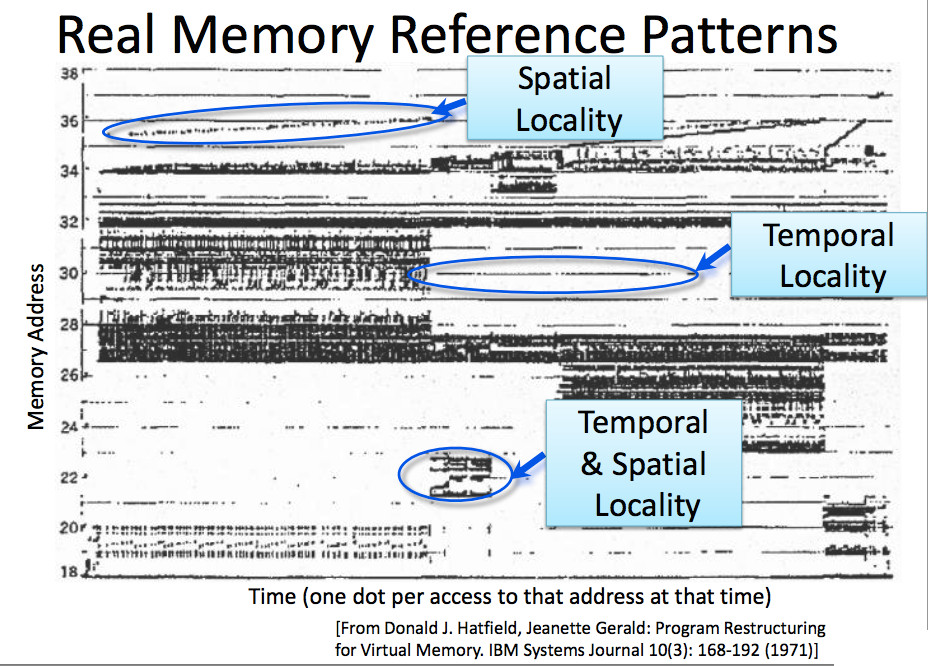
\includegraphics[width=0.9\linewidth]{img/localitygraph.jpg}
		\end{figure}
\end{frame}

%------------------------------------------------

\begin{frame}[plain]
	\frametitle{Human Friendly Memory Locality Graph}
		\begin{figure}
			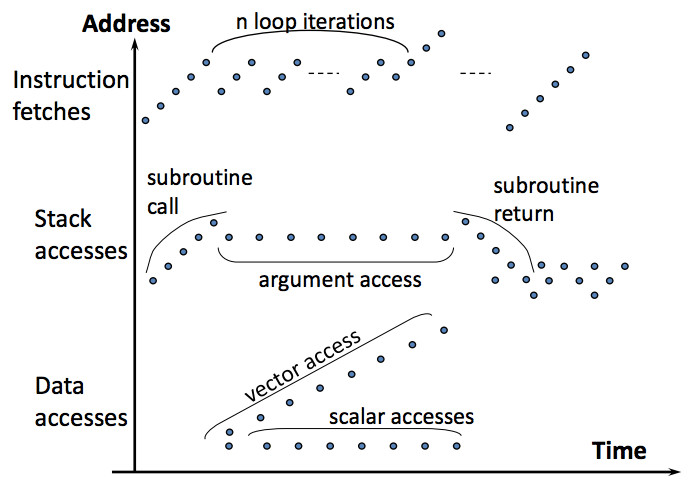
\includegraphics[width=0.9\linewidth]{img/localitygraph2.jpg}
		\end{figure}
\end{frame}

%------------------------------------------------

\begin{frame}[plain]
	\frametitle{Human Friendly Memory Locality Graph}
		\begin{figure}
			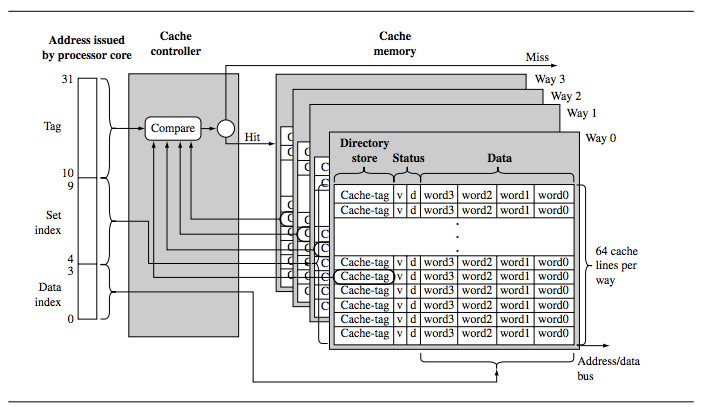
\includegraphics[width=1\linewidth]{img/cacheinternals.jpg}
		\end{figure}
\end{frame}

%------------------------------------------------

\begin{frame}
	\frametitle{The Cache Policies}
	\begin{itemize}
		\item Replacement Policies: LRU, Random, FIFO, Not Recently Used. 
		\item Write Policies: \textbf{Write Back}, Write Through
		\item Allocation Policies: No Write Allocate, Write Allocate
	\end{itemize}

\end{frame}

%------------------------------------------------

\subsection{The Design}
\begin{frame}
	\frametitle{The Design Highlights}
	\begin{itemize}
		\item It plays with rule of cache controller
		\item Each design belongs a specific architecture
		\item Cache size is the most important limitation
		\item We proposed many small gadgets call each other with an order
		\item It inherits the feature of polymorphism.
		\item Body is called smaller gadgets which conserved in cache
		\item Tail will invoke next gadget.
		\item Theoretically, if you work in Ring 0, Nobody can interrupt your process.
		\item In case of interruption, it is still not matter.
	\end{itemize}

\end{frame}

\begin{frame}[plain]
	\frametitle{Our Approaches on the Control Flows}
		\begin{figure}
			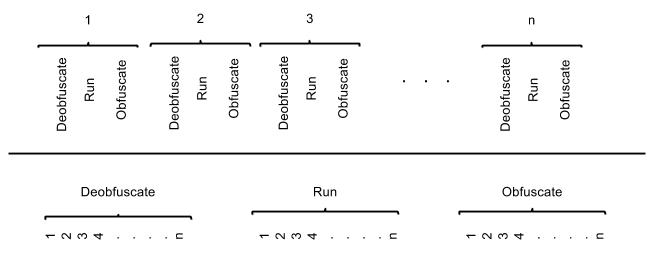
\includegraphics[width=1\linewidth]{img/control_flow.jpg}
			\caption{1. Stepped Approach 2. All in Once Approach}

		\end{figure}
\end{frame}

\subsection{Implementation Issues}
\begin{frame}
	\frametitle{Pitfalls and Fallacies}
	\begin{itemize}
		\item It is too much theoretical.
		\item Cache Coherency is absent.
		\item Real Systems are a lot more complex and indeterministic.
		\item Out-of-Order cpu can brake our stepped approach.
		\item Harvard Architecture leads a problem kind of TLB splitting.
	\end{itemize}
\end{frame}







%------------------------------------------------
\section{Snoopy Cache Coherency Problem}
%------------------------------------------------
\begin{frame}
	\frametitle{The Second Answer}
	\huge{\centerline{Probabilistic Cache Coherency Attack}}
\end{frame}

%------------------------------------------------
\subsection{What It is}
\begin{frame}
	\frametitle{Tightly Coupled Memory Systems}
		\begin{figure}
			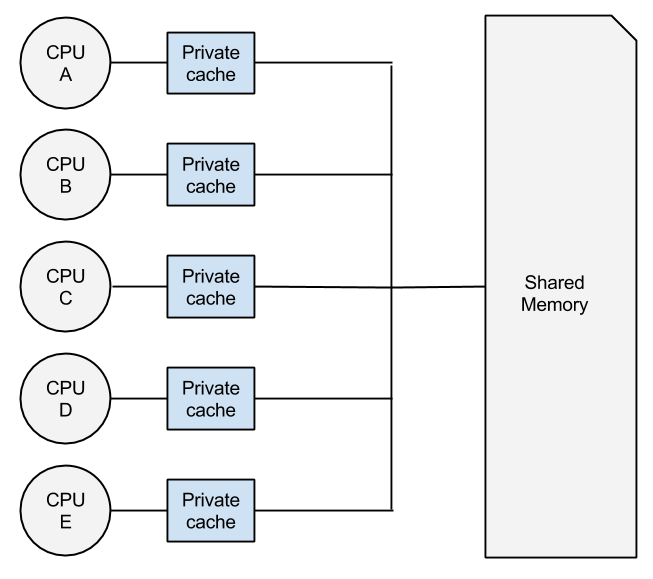
\includegraphics[width=0.6\linewidth]{img/tightly_coupled_memories.png}
		\end{figure}
\end{frame}

%------------------------------------------------
\begin{frame}
	\frametitle{Details about Snoopy Cache Coherency}
	\begin{itemize}
		\item Cache controllers are not simple anymore
		\item There is a network between cache controllers
		\item Each caches are obligated to snoop and log cache states
		\item There are standard protocols to handle coherency with different simplicity levels such as MSI, MESI, MOSI
		\item The systems consume more energy.
		\item Traffic Filters can increase bandwidth enormously.
	\end{itemize}
\end{frame}

%------------------------------------------------
\subsection{Snoopy Coherency Protocols}
\begin{frame}[plain]
	\frametitle{MSI Protocol}
		\begin{figure}
			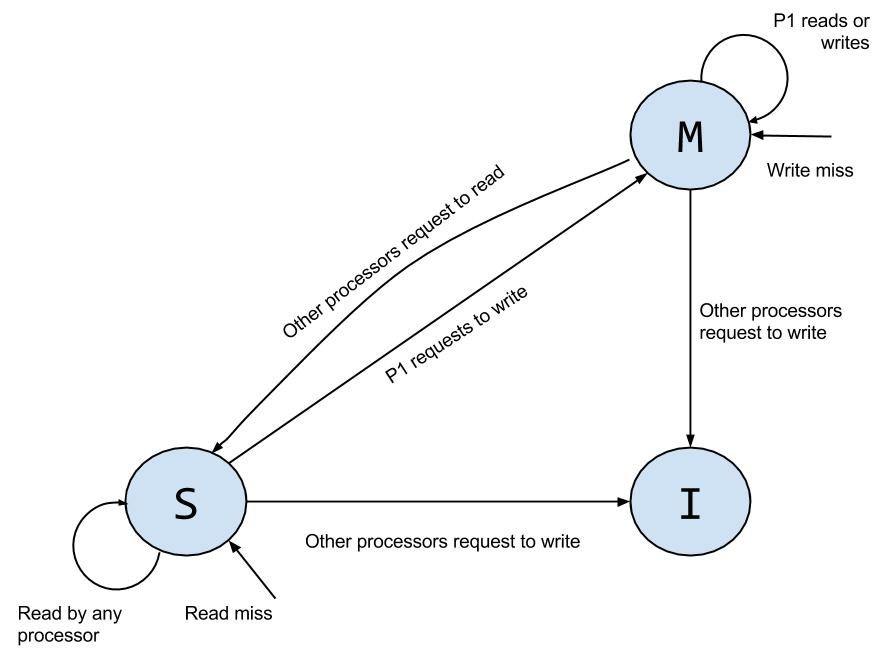
\includegraphics[width=1\linewidth]{img/MSIstatediagram.jpg}
		\end{figure}
\end{frame}

%------------------------------------------------

\begin{frame}[plain]
	\frametitle{MOESI Protocol}
		\begin{figure}
			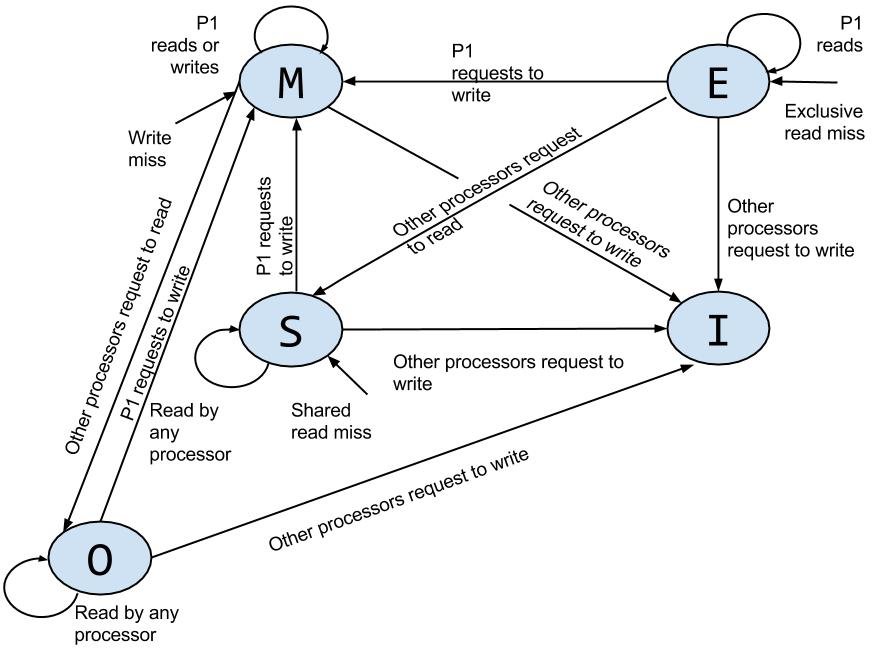
\includegraphics[width=1\linewidth]{img/MOESIstatediagram.jpg}
		\end{figure}
\end{frame}

%------------------------------------------------

\subsection{Snoopy Coherency Weaknesses}
\begin{frame}
	\frametitle{The Dark Side of the Efficiency Optimizations}
	\begin{enumerate}
		\Large
		\item Firm Vertical Line Fetching Direction
		\item The Network Latency
	\end{enumerate}
\end{frame}

%------------------------------------------------

\begin{frame}[plain]
	\frametitle{Firm Vertical Line Fetching Direction}
		\begin{figure}
			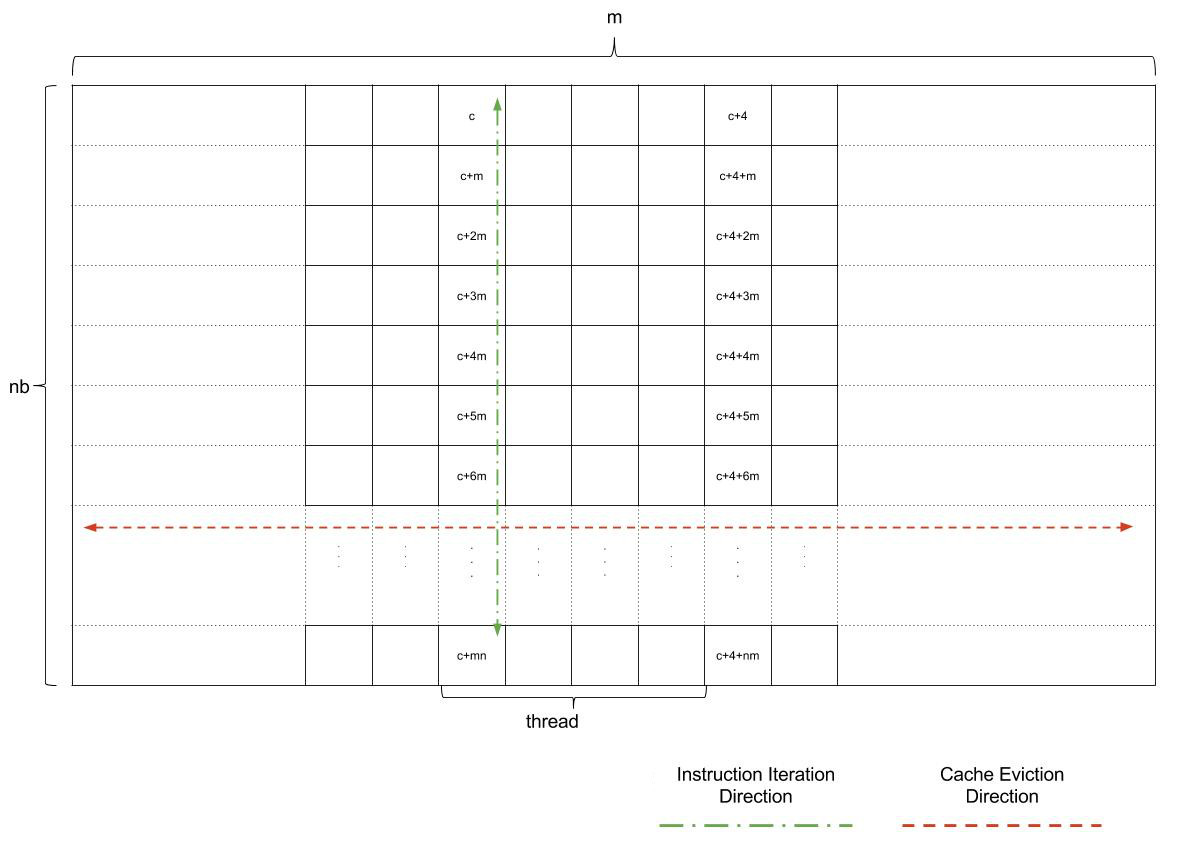
\includegraphics[width=1\linewidth]{img/vertical_instruction_iteration.jpg}
		\end{figure}
\end{frame}

%------------------------------------------------

\begin{frame}[plain]
	\frametitle{The Network Latency}
		\begin{figure}
			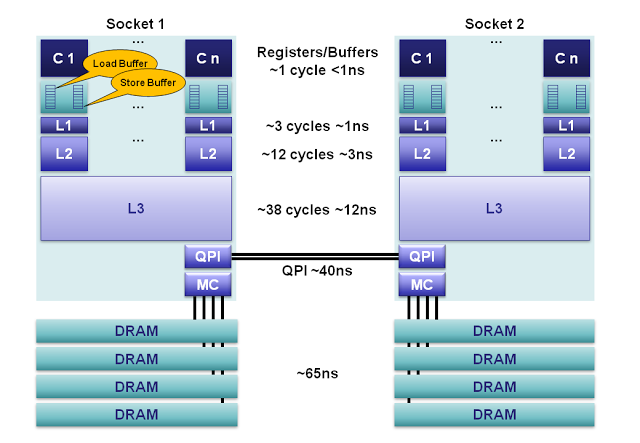
\includegraphics[width=1\linewidth]{img/memory_latency.png}
			\caption{2012 Sandy Bridge Latency illustration by Intel}
		\end{figure}
\end{frame}

%------------------------------------------------

\begin{frame}[plain]
	\frametitle{The Congestion Effect over The Network Latency}
		\begin{figure}
			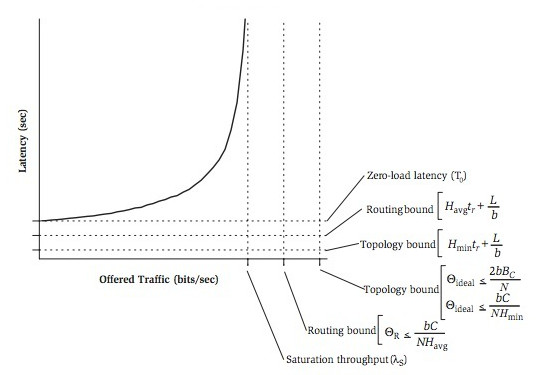
\includegraphics[width=1\linewidth]{img/latency_graph.jpg}
		\end{figure}
\end{frame}

%------------------------------------------------

\subsection{Simulation Results}
\begin{frame}[plain]
	\frametitle{Simulation Topology}
		\begin{figure}
			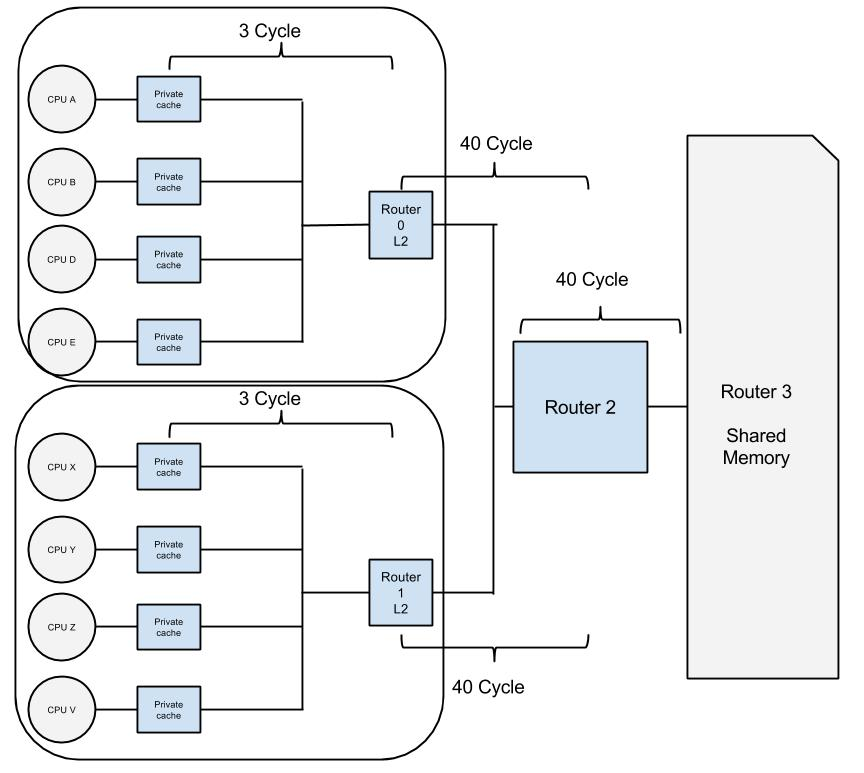
\includegraphics[width=0.8\linewidth]{img/simulation.jpg}
		\end{figure}
\end{frame}

%------------------------------------------------
\begin{frame}
	\frametitle{Latency Simulation Results}
\begin{table}[h]
	\small
\begin{tabular}{|l|c|c|c|c|}
	\hline
                  & \begin{tabular}[c]{@{}c@{}}Packet latency\\ Min/Avg/Max\end{tabular} & \begin{tabular}[c]{@{}c@{}}Network latency\\ Min/Avg/Max\end{tabular} & \begin{tabular}[c]{@{}c@{}}Flit latency\\ Min/Avg/Max\end{tabular} \\ \hline
Crowded 2\%            & 164/68045/171627                                                     & 13/417/1487                                                           & 13/353/1487                                                       \\ \hline
Small 2\%            & 8/72/216                                                             & 8/72/216                                                              & 8/72/216                                                          \\ \hline
Crowded 4\%            & 15698/178598/458108                                                  & 13/410/1736                                                           & 13/353/1736         \\ \hline
Small 4\%            & 8/322/1273                                                           & 8/129/376                                                             & 8/129/376        \\ \hline
\end{tabular}
\end{table}
\end{frame}

%------------------------------------------------

\subsection{Our Probabilistic Attack}
\begin{frame}
	\frametitle{The Essences of Our Attack}
	 \begin{itemize}
	 	\item Horizontal Arrangement except stub section
	 	\item Lazy Cache Protocol 
	 	\item It is as obfuscated as how late the network is.
	 \end{itemize}
\end{frame}

%------------------------------------------------

\begin{frame}
	\frametitle{Horizantal Arrangement}
\begin{exampleblock}{Arrangement Formula}
\[
	I(i)=m*(i\bmod{(nb)})+((\left \lfloor i/nb \right \rfloor*thread)+c)\bmod{m}
\]
\end{exampleblock}
\begin{exampleblock}{Bijection condition}
\[
	\forall\: m\bmod thread = 1\ :\  I()\ is\ bijective\ function
\]
\end{exampleblock}
\end{frame}

\subsection{Simulation Results}
\begin{frame}[plain]
	\frametitle{Simulation Topology}
		\begin{figure}
			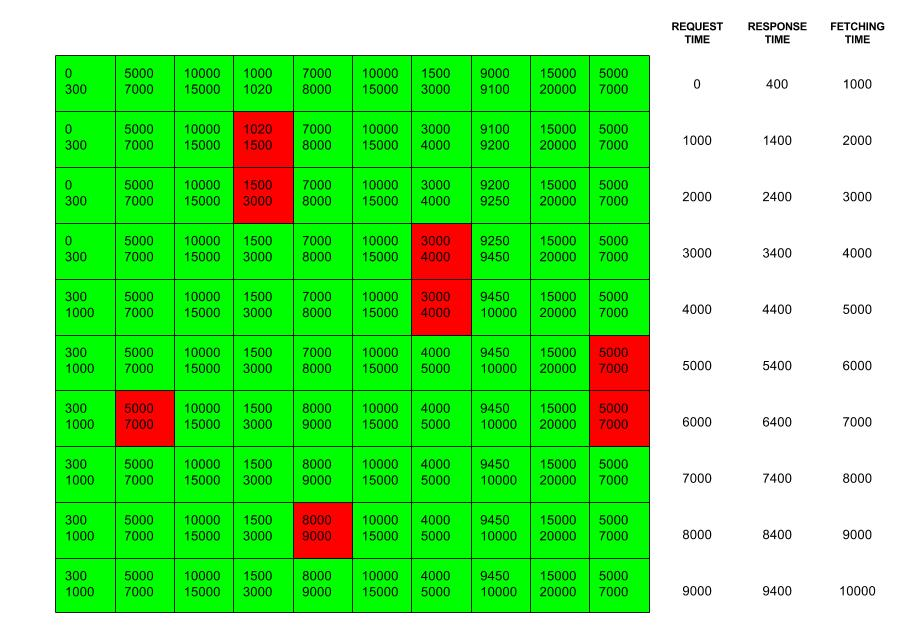
\includegraphics[width=1.1\linewidth]{img/overall_timing_attack.jpg}
		\end{figure}
\end{frame}


%------------------------------------------------
\section{Harvard Architecture Problem}
%------------------------------------------------
\begin{frame}
	\frametitle{The Third Answer}
	\huge{\centerline{Flying Over Interpreter}}
\end{frame}
%------------------------------------------------

\subsection{Harvard Architecture}
\begin{frame}
	\frametitle{Harvard Architecture}
		\begin{figure}
			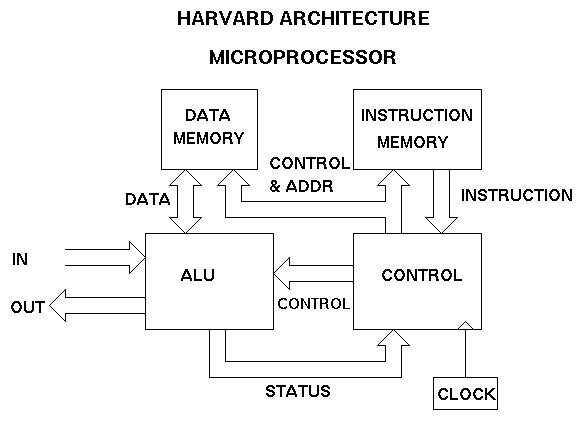
\includegraphics[width=0.75\linewidth]{img/harvard.png}
		\end{figure}
\end{frame}

%------------------------------------------------

\subsection{Our Solution}
\begin{frame}
	\frametitle{Harvard Architecture}
		\begin{figure}
			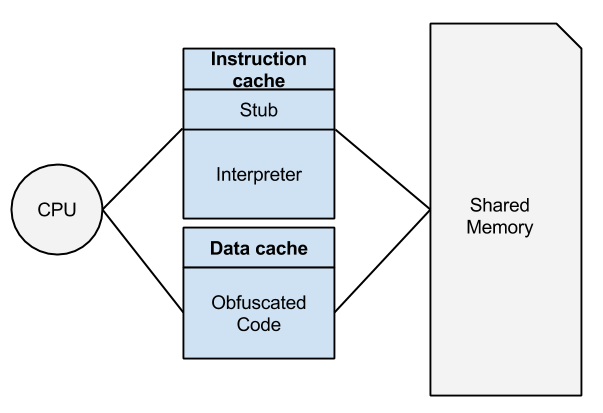
\includegraphics[width=0.75\linewidth]{img/Harvard_implementation.png}
		\end{figure}
\end{frame}

%------------------------------------------------

\begin{frame}
	\frametitle{Flying over Interpreter}
	\begin{itemize}
		\item Sparks, S. \& Butler, J. 2005. Shadow walker
		\item Yan, W., Zhang, Z., \& Ansari, N. 2008. Revealing packed malware
		\item FORTH Language is a treasury legitimate interpreter
		\item Instead of executing instruction, we will interrupt script a language.
	\end{itemize}
\end{frame}

%------------------------------------------------








%------------------------------------------------
\section{Ending}
%------------------------------------------------
	\subsection{Realisation and Implementation Issues}
%------------------------------------------------




%------------------------------------------------

\begin{frame}
	\frametitle{Conclusion}
	\begin{itemize}
		\item Detection methods must be discussed in another work.
		\item New architectures are always tricky.
		\item However, with increasing deployment of multi-processor computing and other parallel processing devices, the implementation of local memories like NUMA and caches are increasing in order to increase efficiently and performance and decrease power consumption. 
		\item It is obviously clear that these features will also be exploited by malware authors at some point. 
	\end{itemize}
\end{frame}

%------------------------------------------------

\begin{frame}
	\frametitle{What is solution?}
	\begin{figure}
		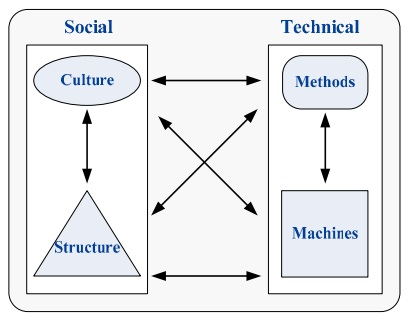
\includegraphics[width=0.8\linewidth]{img/sociatech.jpg}
	\end{figure}
\end{frame}

\begin{frame}
	\frametitle{Acknowledgements}
	\Large{\centerline{Prof. Stephen Wolthusen and Emre Tinaztepe}}
\end{frame}

\begin{frame}
	\frametitle{Thanks}
	\Huge{\centerline{Thank You}}
\end{frame}



%------------------------------------------------

\begin{frame}
	\Huge{\centerline{The End}}
	\centerline{and}
	\Huge{\centerline{Questions}}
\end{frame}

%----------------------------------------------------------------------------------------

\end{document} 